\documentclass[a11paper, 11pt]{article}
% xelatex

\usepackage[T1]{fontenc}
\usepackage{inputenc}
\usepackage[style=ieee]{biblatex}
\usepackage{libs/document}
\usepackage{libs/titlepage}
\usepackage{booktabs}
\usepackage{subcaption}
\usepackage[american]{circuitikz}
% \usepackage{showframe}
\usepackage{float}
\usepackage{multicol}
\usepackage{siunitx}
\usepackage[dvipsnames]{xcolor}
\usepackage{csquotes}
\usepackage[french]{babel}
\usepackage{hyperref}
\usepackage[french]{cleveref}

\newcommand{\todo}[1]{\begin{color}{Red}\textbf{TODO:} #1\end{color}}
\newcommand{\note}[1]{\begin{color}{Orange}\textbf{NOTE:} #1\end{color}}
\newcommand{\fixme}[1]{\begin{color}{Fuchsia}\textbf{FIXME:} #1\end{color}}
\newcommand{\question}[1]{\begin{color}{ForestGreen}\textbf{QUESTION:} #1\end{color}}

\DeclareNameAlias{author}{family-given}
\addbibresource{refs/references.bib}

\DeclareSIPrefix{\micro}{%
  \text{%
    \fontencoding{TS1}\fontfamily{kurier}\selectfont
    \symbol{"B5}%
  }%
}{-6}

\begin{filecontents*}[overwrite]{zoumbadouwow.bib}
@misc{yellow-led,
  title = {{YELLOW} {LED} - {Everlight} {Americas} {Inc}.},
  url = {
         https://everlightamericas.com/through-hole-led-lamps/1893/EALP05RDHYA0.html?search_query=EALP05RDHYA0&results=1
         },
  language = {English},
  urldate = {2024-10-15},
  journal = {Through Hole LED Lamps -},
  author = {{Everlight Americas Inc.}},
  file = {PDF:/home/zaikos/Zotero/storage/GRH7TTIR/Through Hole LED Lamps -
          Everlight Americas Inc..PDF:application/pdf;YELLOW LED - Everlight
          Americas
          Inc.:/home/zaikos/Zotero/storage/N7IK9FU8/EALP05RDHYA0.html:text/html},
}

@misc{blue-led,
  title = {{BLUE} {LED} - {Everlight} {Americas} {Inc}.},
  url = {
         https://everlightamericas.com/through-hole-led-lamps/1810/ealp05rddba3.html
         },
  urldate = {2024-10-15},
  journal = {Through Hole LED Lamps -},
  author = {{Everlight Americas Inc.}},
  file = {PDF:/home/zaikos/Zotero/storage/GH3R2W68/Everlight Americas Inc. -
          BLUE LED - Everlight Americas Inc..PDF:application/pdf;Through Hole LED
          Lamps - Everlight Americas
          Inc.:/home/zaikos/Zotero/storage/6KC7JDMH/ealp05rddba3.html:text/html},
}
\end{filecontents*}

\addbibresource{zoumbadouwow.bib}
% \institution{Université de Sherbrooke}
% \faculty{Faculté de génie}
% \department{Département de génie électrique et de génie informatique}
\title{Rapport d'APP}
\class{Circuits électriques I\\Circuits électriques II\\La communication et le travail en équipe}
\classnb{GEN135\\GEN136\\GEN111}
\author{
  \addtolength{\tabcolsep}{-0.4em}
  \begin{tabular}{rcl} % Ajouter des auteurs au besoin
      Benjamin Chausse & -- & CHAB1704 \\
      Sarah Gosselin   & -- & GOSS3005 \\
  \end{tabular}
}
\teacher{Jean-Philippe Gouin}
% \location{Sherbrooke}
% \date{\today}

\begin{document}
\maketitle
\newpage
\tableofcontents
\newpage

\section{Introduction}

Dans le cadre du défi du combatant, le robot ROBUS devra être capable de se déplacer avec
un suiveur de ligne. Celui fourni par l'Université est composé de trois phototransistors
détectant le blanc à une distance de \SI{4}{\mm} qui déclenchent chacun un ampli-OP branché
en mode comparateur et qui génère une tension unique lorsque activé. À titre d'indication,
trois DELs (rouge, jaune, et bleu) sont utilisées pour indiquer l'état des phototransistors.
La somme des tensions générées par les ampli-OP est enfin normalisée par un ampli-OP additionnel
configuré en mode comparateur afin que le courant maximal en sortie (lu par un microcontrôleur)
soit de \SI{5}{\V}. Toutefois, le circuit fourni a des valeurs de résistances manquantes, il est
donc nécessaire de les déterminer de façon calculée, simulée, et expérimentale afin que le
circuit se comporte dans les limites attendues.


\section{Déterminer la valeur de $R_3$}
\label{sec:first-res}

\begin{multicols}{2}
	Dans le contexte de notre circuit, le transistor opère en mode saturé. Selon
	la fiche de spécifications du fabricant, il y a une différence de potentiel
	de \SI{0.2}{V} entre la borne du collecteur et celle de l'émetteur dans ce
	mode de fonctionnement. Aussi, le guide étudiant énonce qu'un minimum
	de \SI{10}{\m\ampere} est nécessaire au fonctionnement de la diode $D_1$.
	Toutefois ce n'est qu'un minimum et la spécification de la diode recommande
	un courant de \SI{20}{\m\ampere} lors d'une utilisation standard. À ce
	courant précis, une différence de potentiel de \SI{2}{\V} est observé
	(encore une fois selon la spécification). Enfin, la quantité de courant
	passant de la base du transistor à l'émetteur est quasi-nulle. Elle sera
	donc négligée. Le système est alors composé d'une seule boucle où toutes
	les composantes sont en série.

	\columnbreak
	\begin{figure}[H]
		\centering
		\begin{circuitikz}
			\node at (-0.5,3) (src) {5V};

			\node[npn] at (4,1) (npn) {}
			(npn.base) node[anchor=east] {$Q_1$} % B
			(npn.collector) node[anchor=north] {} % C
			(npn.emitter) node[anchor=south] {}; % E
			\draw (npn) circle (0.85cm);

			\draw (npn.emitter) to (4,0) node[ground] {} ;

			\draw (src) to[R,l=$R_3$,i=$I$] (2,3)
			to[led,l=$D_1$]        (4,3)
			to (npn.collector);

		\end{circuitikz}
		\caption{Circuit pour $D_1$ controllé via $Q_1$}
	\end{figure}
\end{multicols}

\begin{gather}
	I             = 20\times10^{-3} \si{\ampere},\quad
	V_{D_1}       = 2 \si{\V},\quad
	V_{Q_1}       = 0.2 \si{\V},\quad
	V_{CC}        = 5 \si{\V}                   \\
	V_{R_3}       = R_3 I                       \\
	V_{CC}        = V_{R_3} + V_{D_1} + V_{Q_1} \\
	V_{CC}        = R_3 I + V_{D_1} + V_{Q_1}   \\
	R_3 = \frac{V_{CC}- V_{D_1} - V_{Q_1}}{I}   \\
	% 5            = R_3 20\times10^{-3} + 2 + 0.2   \\
	R_3 = \frac{5\si{\V} - 2\si{\V} - 0.2\si{\V}}{20\times10^{-3}\si{\ampere}}
	= 140\si{\ohm}
\end{gather}

\section{Courant circulant dans les DEL bleue et jaune}

En analysant les sous-circuit des diodes $D_2$ (jaune) et $D_3$ (bleue) avec
la méthode de Thévenin Norton, on remarque que chaque circuit est capable
d'opérer à une tension maximale et avec un courant maximal respectifs.
Puisque le sous-circuit contient un transistor qui a une tension de
\SI{0.2}{\V} entre sont émetteur et son collecteur en mode saturation (voir
\cref{sec:first-res}), une tension de \SI{4.8}{\V} est posée au lieu de
\SI{5}{\V} pour Thévenin Norton. En comparants les contraintes de chacun des
circuits à la spécification des leur diode associée par la méthode de charge,
il est alors possible de déterminer le courant et la tension parcourant les
DEL. $D_2$ opère à un courant de \SI{10}{\milli\ampere} avec une tension de
\SI{1.8}{\V} alors que $D_3$ opère avec un courant de \SI{7.5}{\milli\ampere}
et une tension de \SI{2.8}{\V} entre ses bornes.

\begin{figure}[H]
	\begin{subfigure}{0.4\textwidth}
		\centering
		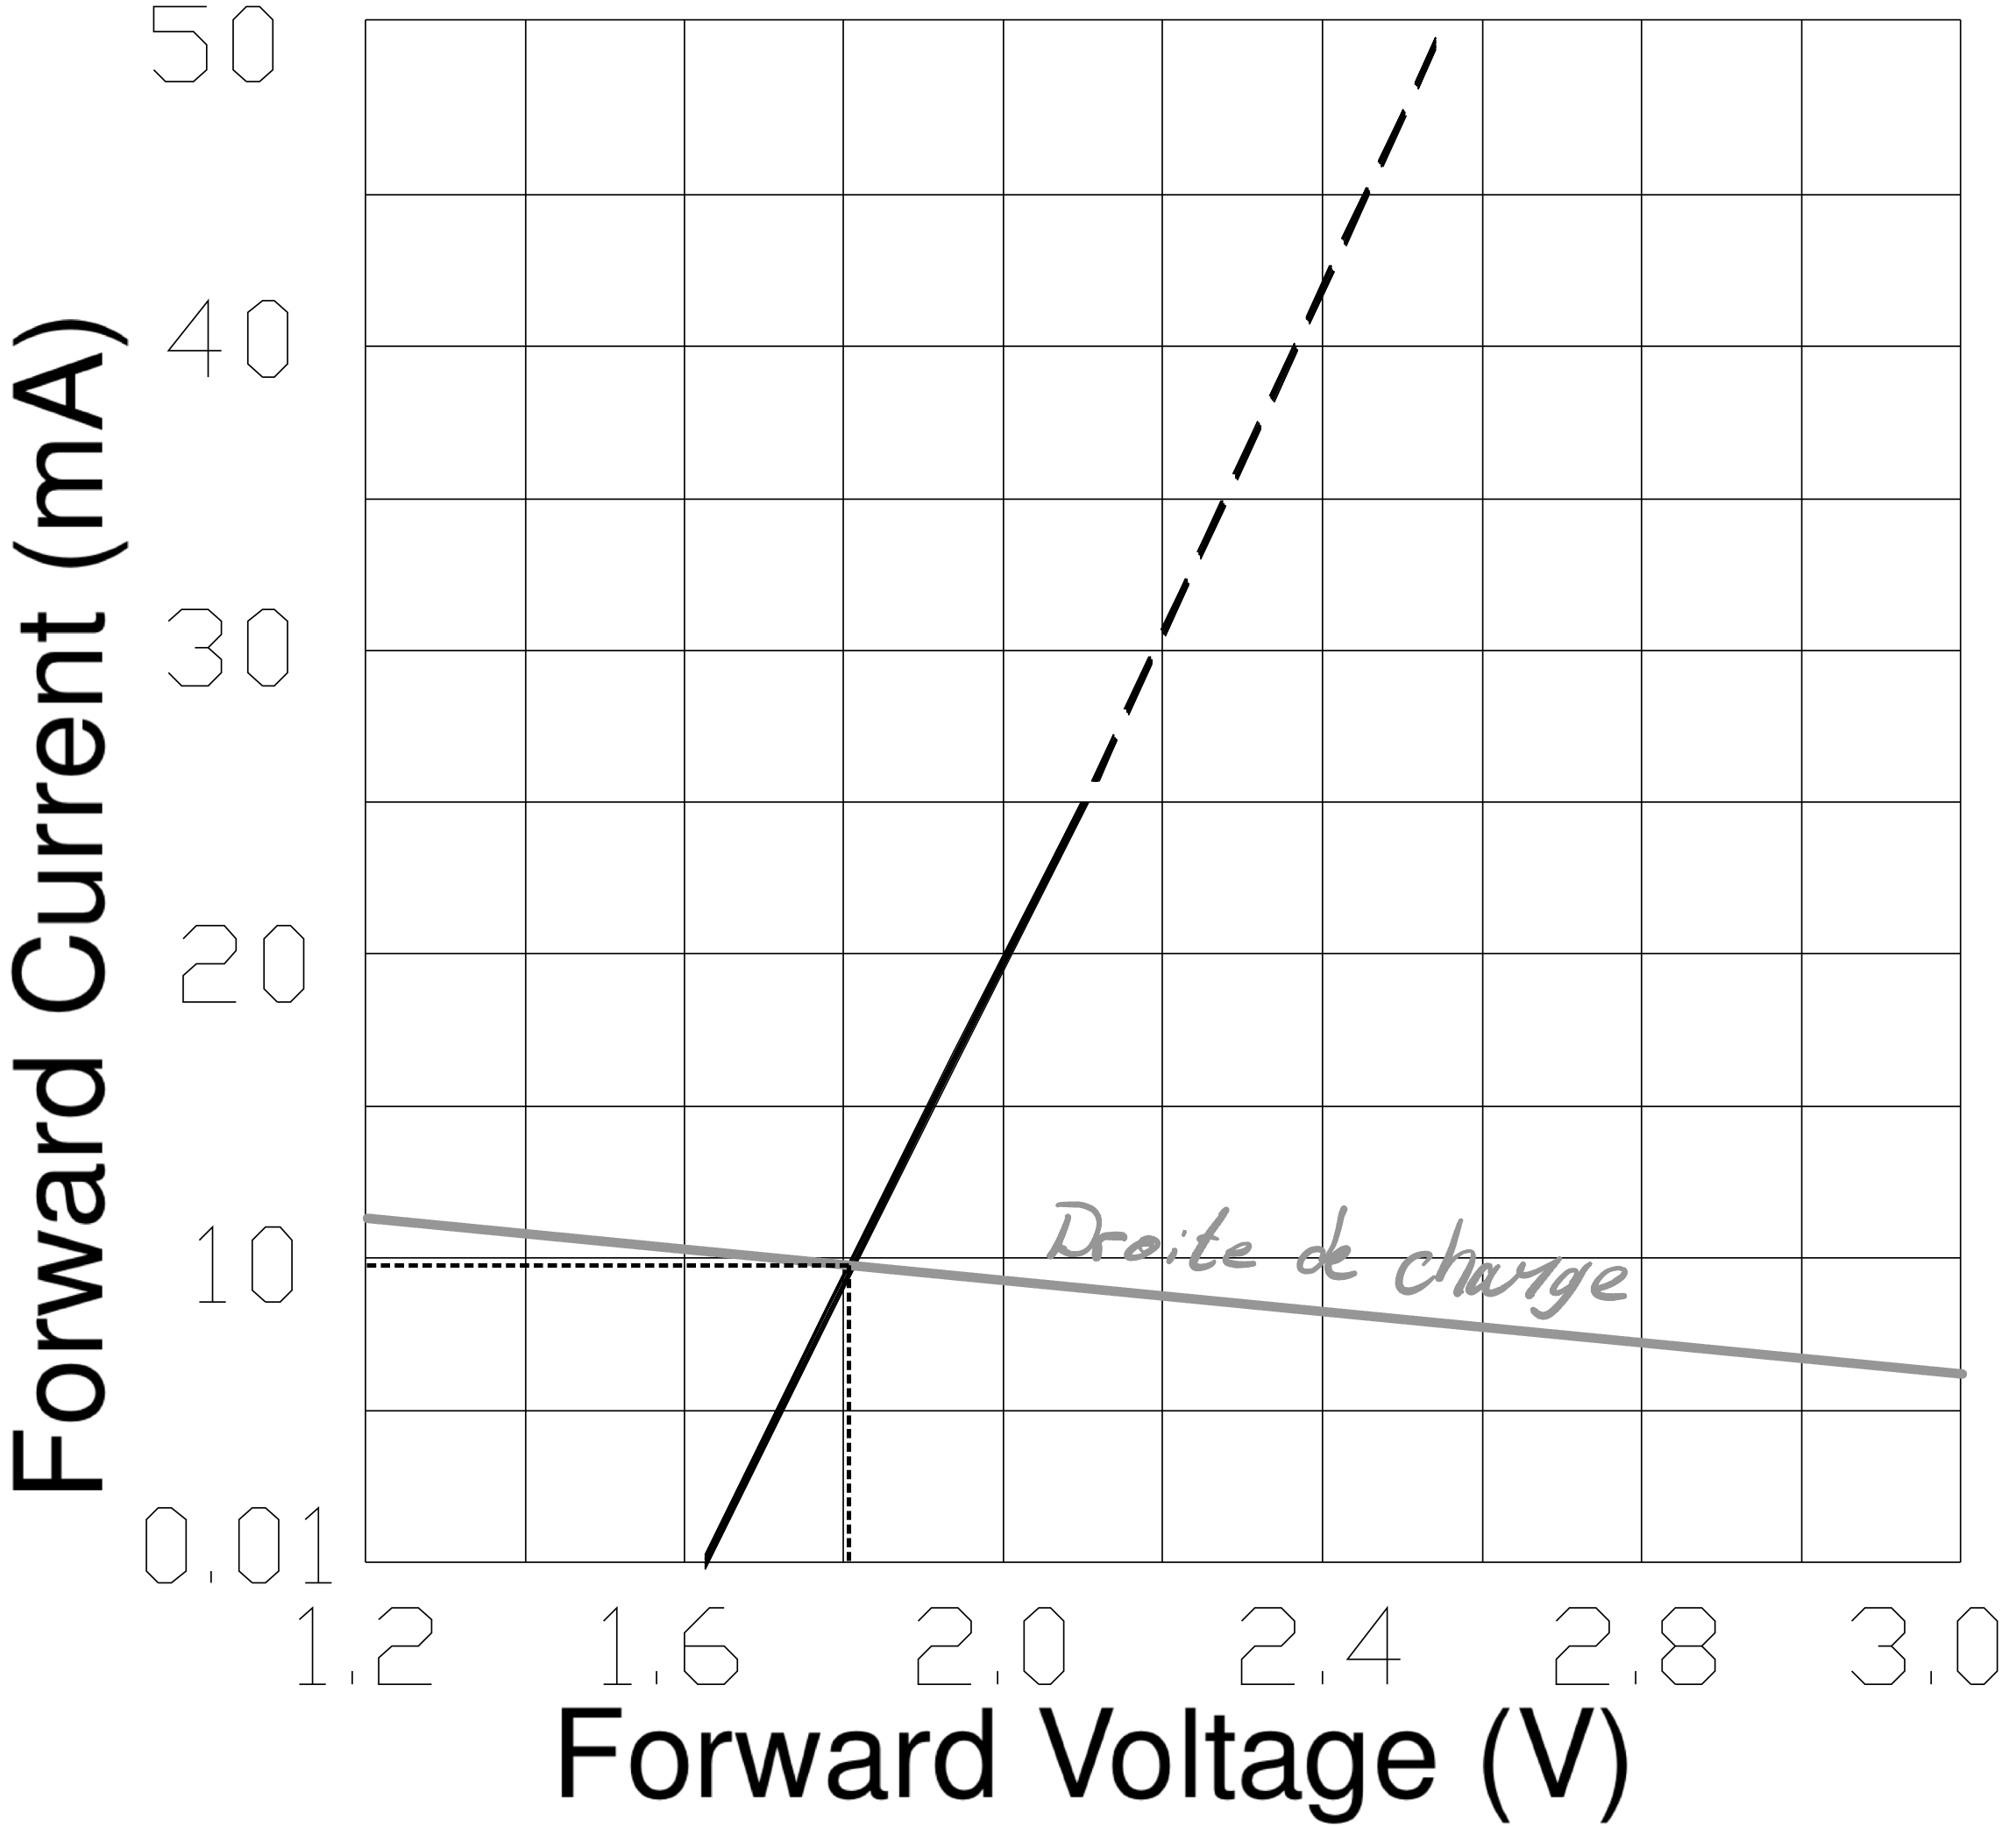
\includegraphics[width=\textwidth]{figures/yellow.png}
		\caption{Diode $D_2$ \cite{yellow-led}}
		\label{subfig:yellow}
	\end{subfigure}
	\hfill
	\begin{subfigure}{0.4\textwidth}
		\centering
		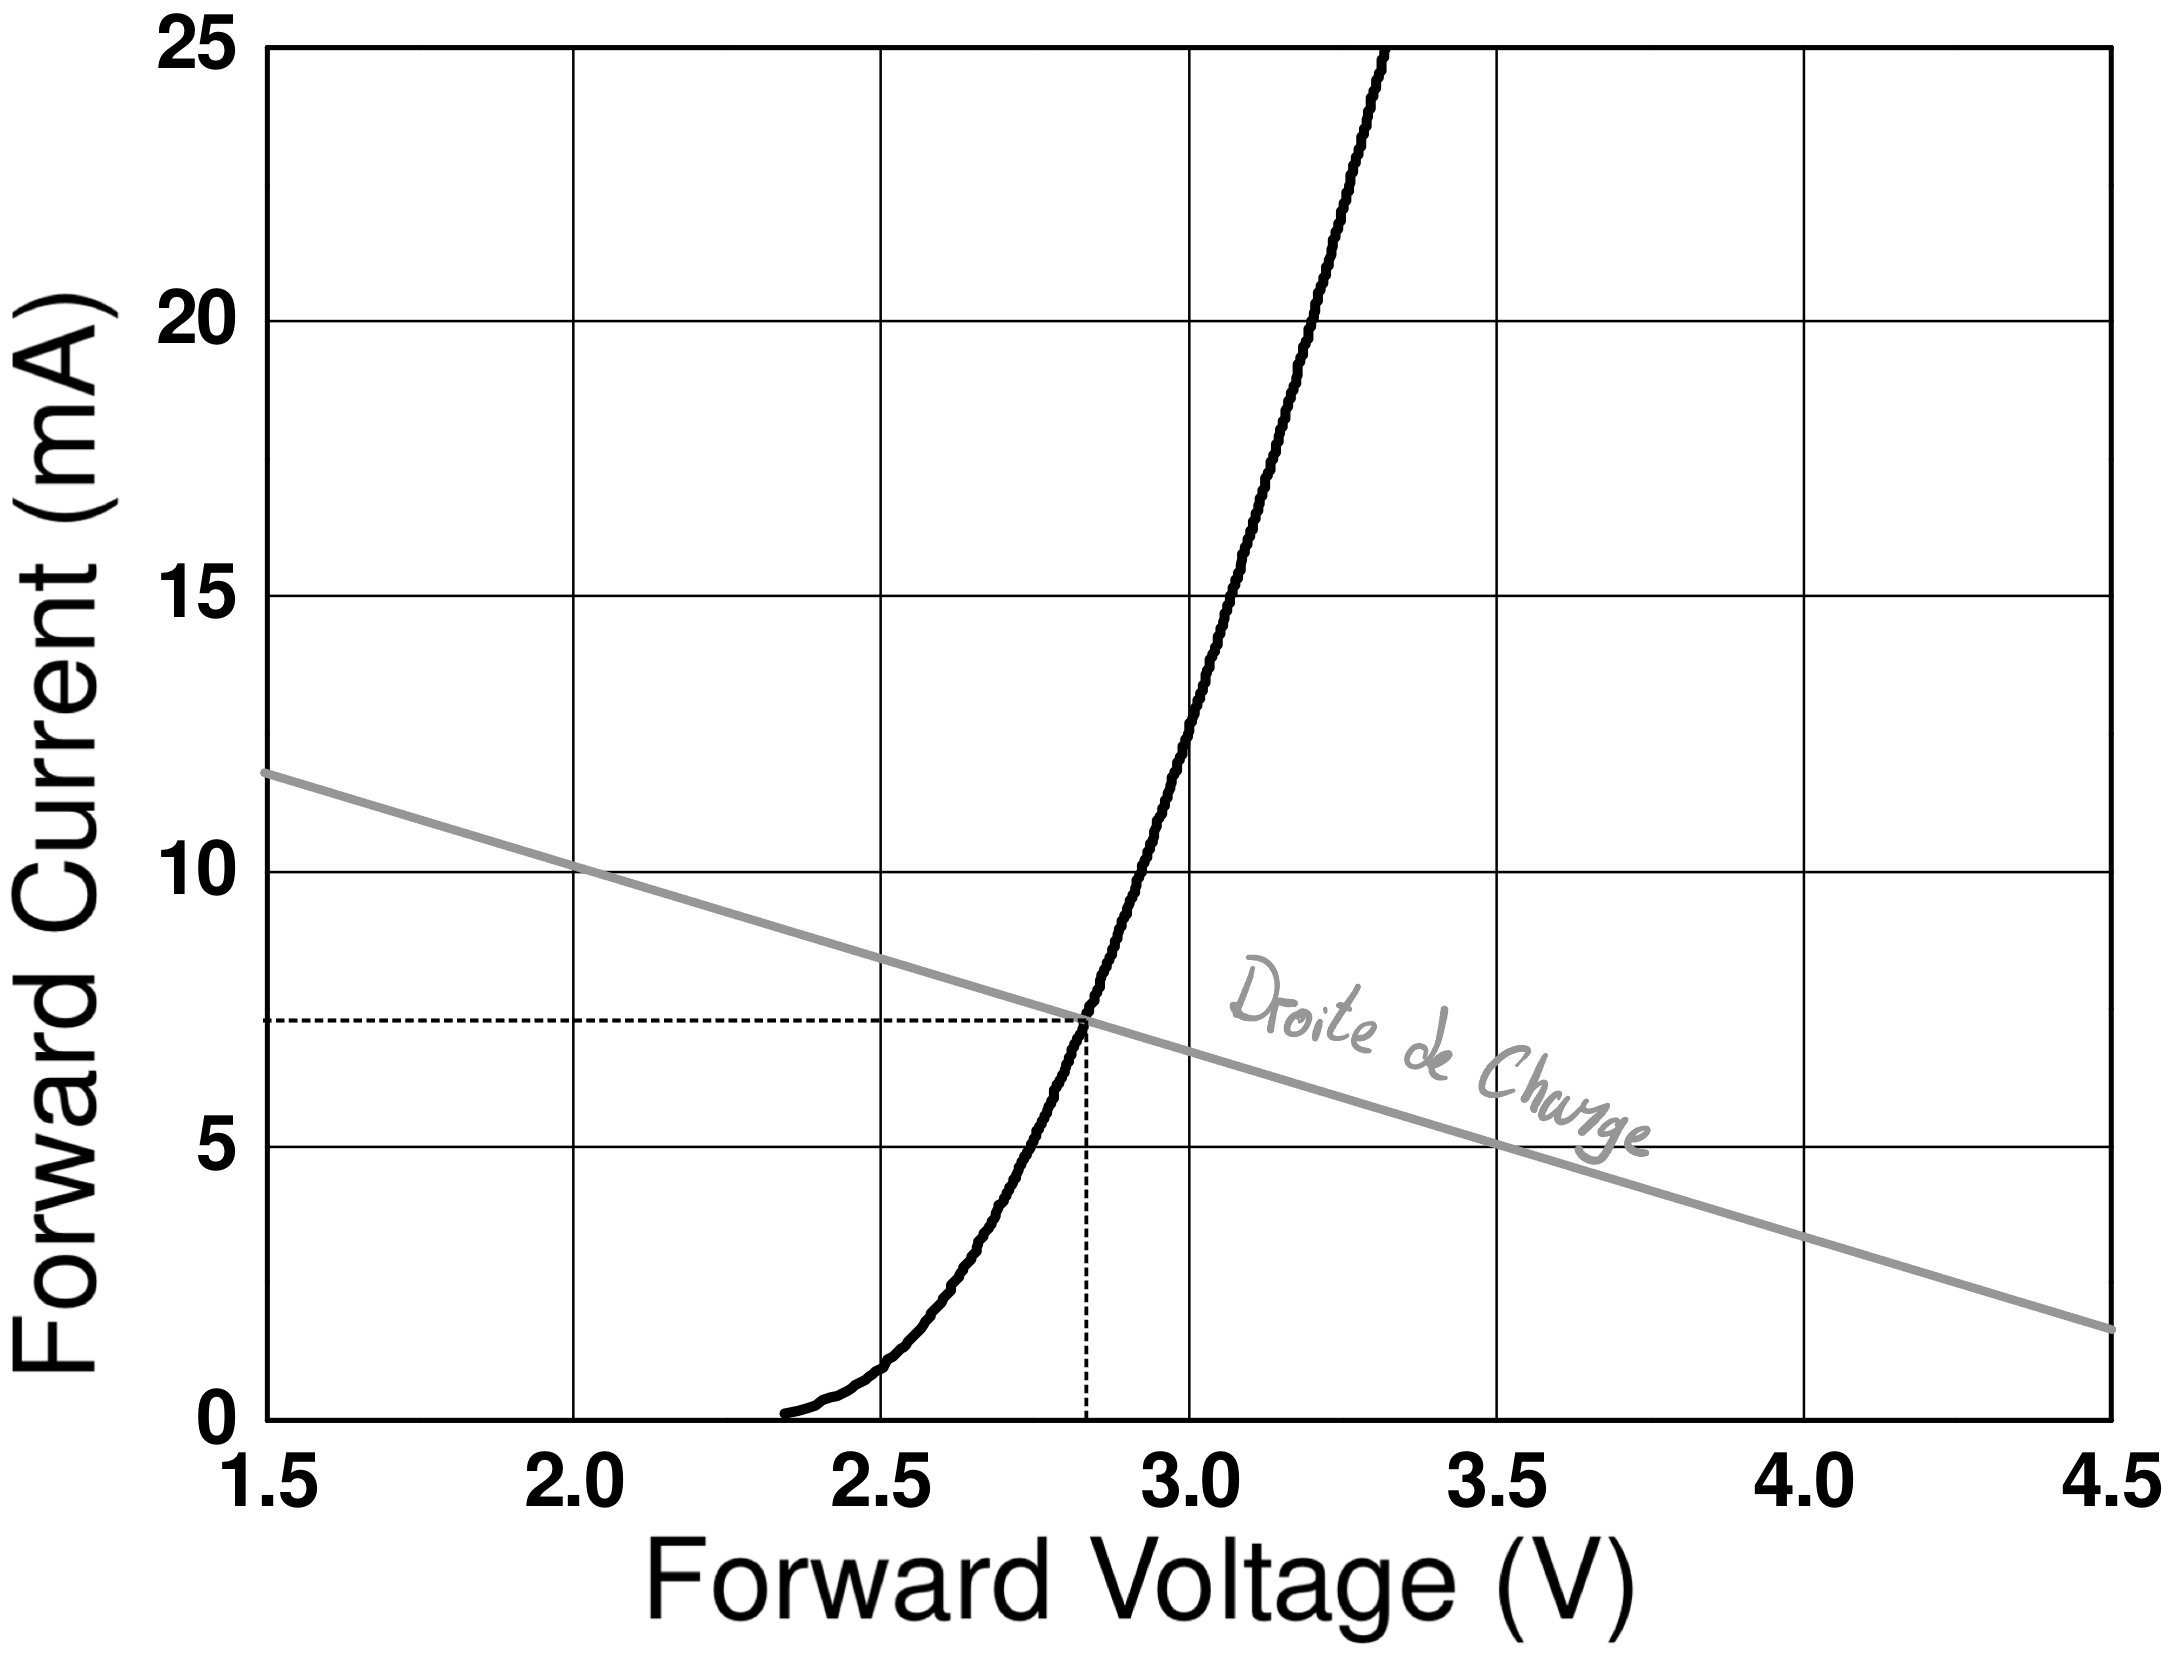
\includegraphics[width=\textwidth]{figures/blue.png}
		\caption{Diode $D_3$ \cite{blue-led}}
		\label{subfig:blue}
	\end{subfigure}
	\caption{Intesection des droites de charge des diodes}
\end{figure}


\section{Analyse du circuit simplifié de l'additionneur}

\subsection{Mise en équation par la méthode des boucles}
\begin{gather}
	V_1 = R_{13}i_1 + R_{14}(i_1-i_2) + V_2 \\
	V_2 = R_{14}(i_2 - i_1) + R_{15}(i_2-i_3) + V_3 \\
	V_3 = R_{15}(i_3 - i_2) + R_{16} i_3
\end{gather}

\subsection{Mise en équation par la méthode des n\oe uds}
\begin{gather}
	I_{\textrm{total}}   = I_1 + I_2 + I_3 \label{eq:sumOfI}   \\
	\frac{V_{out}}{R_{16}} = \frac{V_1-V_{out}}{R_{13}} +
	\frac{V_2-V_{out}}{R_{14}} + \frac{V_3-V_{out}}{R_{15}} \\
	V_{out} = \frac{\frac{V_1}{R_{13}}+\frac{V_2}{R_{14}}+\frac{V_3}{R_{15}}}
	{\frac{1}{R_{13}}+\frac{1}{R_{14}}+\frac{1}{R_{15}}+\frac{1}{R_{16}}} \label{eq:vOut-symb}
\end{gather}


\subsection{Mise en équation par la méthode de superposition}
\begin{gather}
	V_{out_1} = V_1\left(\frac{\big(\frac{1}{R_{14}}+\frac{1}{R_{15}}+\frac{1}{R_{16}}\big)^{-1}}
	{R_{13}+\big(\frac{1}{R_{14}}+\frac{1}{R_{15}}+\frac{1}{R_{16}}\big)^{-1}}\right) \\
	V_{out_2} = V_2\left(\frac{\big(\frac{1}{R_{13}}+\frac{1}{R_{15}}+\frac{1}{R_{16}}\big)^{-1}}
	{R_{14}+\big(\frac{1}{R_{13}}+\frac{1}{R_{15}}+\frac{1}{R_{16}}\big)^{-1}}\right) \\
	V_{out_3} = V_3\left(\frac{\big(\frac{1}{R_{13}}+\frac{1}{R_{14}}+\frac{1}{R_{16}}\big)^{-1}}
	{R_{15}+\big(\frac{1}{R_{13}}+\frac{1}{R_{14}}+\frac{1}{R_{16}}\big)^{-1}}\right)
\end{gather}

\newpage
\subsection{Résolution par la méthode choisie}
\begin{multicols}{2}

	La méthode de résolution choisie est la méthode de n\oe uds.
	En partant de la série d'\crefrange{eq:sumOfI}{eq:vOut-symb},
	il est possible de simplifier en substituant les valeurs des
	résistances $R_{13}$, $R_{14}$, $R_{15}$ et $R_{16}$ afin d'arriver à l'\cref{eq:vOut}.
	Cela permet de trouver des valeurs de $V_{out}$ en fonction des diffentes combinaisons de $V_n$.

	\columnbreak

	\begin{figure}[H]
		\centering
		\begin{circuitikz}
			\draw (2,6) to[R,l=$R_{13}$,i_=$I_1$] (4,6);
			\draw (2,4) to[R,l=$R_{14}$,i_=$I_2$] (4,4);
			\draw (2,2) to[R,l=$R_{15}$,i_=$I_3$] (4,2);

			\draw (2,6) to[voltage source,l=$V_1$] (0,6);
			\draw (2,4) to[voltage source,l=$V_2$] (0,4);
			\draw (2,2) to[voltage source,l=$V_3$] (0,2);

			\draw (0,6) to(0,2) node[ground] {};

			\draw (4,6) to (4,2) to[R,l_=$R_{16}$,i=$I_{\textrm{total}}$] (6,2) node[ground] {};
			\draw (4,6) to[short, -o,i_=$I_{out}$] (6,6) node[short] {\hspace{.8cm}$V_{\textrm{out}}$};
		\end{circuitikz}
		\caption{Circuit additionneur}
		\label{circ:sum}
	\end{figure}

\end{multicols}

\begin{gather}
	I_{\textrm{out}}     = \SI{0}{\ampere},\quad
	R_{13} = \SI{10}{\kilo\ohm},\quad R_{14} = \SI{20}{\kilo\ohm},
	\quad R_{15} = \SI{40}{\kilo\ohm} \\
	V_{out} = \frac{\frac{V_1}{\SI{10}{\kilo\ohm}}+
		\frac{V_2}{\SI{20}{\kilo\ohm}}+\frac{V_3}{\SI{40}{\kilo\ohm}}}
	{\frac{1}{\SI{10}{\kilo\ohm}}+\frac{1}{\SI{20}{\kilo\ohm}}+
		\frac{1}{\SI{40}{\kilo\ohm}}+\frac{1}{\SI{80}{\kilo\ohm}}} \\
	V_{out} = \frac{8V_1}{15}+\frac{4V_2}{15}+\frac{2V_3}{15} \label{eq:vOut}
\end{gather}



\section{Valeur de $R_{18}$ pour le circuit d'amplification}

\begin{multicols}{2}
	La tension maximale à la sortie du circuit doit être de \SI{5}{\V}. Toutefois,
	la sortie du sommateur donne un gain calculé maximal de $4,\overline{66}\si{\V}$.
	Un Ampli-OP est donc utilisé pour bonnifier le gain maximal (gardant les
	autres gains possibles proportionels). Dans le contexte du diviseur de tension,
	$V_{\textrm{out}}$ correspond à l'entrée du diviseur de tension. Suivant cette
	logique, la sortie du diviseur de tension est nommée $V_{\textrm{retro}}$
	puisqu'elle est branchée de façon à permettre la rétroaction.

	\columnbreak
	\begin{figure}[H]
		\centering
		\begin{circuitikz}
			\node at (-0.1,1.2) (src) {5V};
			\node at (3,0) (out) {$V_{\textrm{out}}$};

			\draw (0,0) node[op amp] (opamp) {}
			(opamp.down) node[ground] {}
			(opamp.-) node[left] {$V_{\textrm{retro}}$}
			(opamp.+) node[left] {$V_{\textrm{sum}}$} ;
			\draw (opamp.up) to (src);
			\draw (opamp.out) to (out);

			\draw (opamp.-) to (-1.2,3)
			to[R,l_=$R_{18}$] (1.7,3) to (1.7,0);

			\draw (-1.2,3) to[R,l^=$R_{17}$] (-3.5,3) node[ground] {};
		\end{circuitikz}
		\caption{Circuit d'amplification}
		\label{circ:amp}
	\end{figure}
\end{multicols}

\begin{align}
	R_{17}=\SI{100}{\kilo\ohm}, & \quad V_{\textrm{sum MAX}}=4,\overline{66}\si{\V}               \\
	V_{\textrm{sum MAX}}        & = V_{\textrm{retro}}                                            \\
	V_{\textrm{retro}}          & = V_{\textrm{out}} \frac{R_{17}}{R_{18}+R_{17}}                 \\
	R_{18}+R_{17}               & = V_{\textrm{out}} \frac{R_{17}}{V_{\textrm{retro}}}            \\
	R_{18}                      & = V_{\textrm{out}} \frac{R_{17}}{V_{\textrm{retro}}}-R_{17}     \\
	R_{18}                      & = \SI{5}{\V} \frac{\SI{100}{\kilo\ohm}}{4.\overline{66}\si{\V}}
	- \SI{100}{\kilo\ohm} = \SI{7.1}{\kilo\ohm}
\end{align}

\section{Résultats et pièces choisies}

\begin{table}[H]
	\centering
	\caption{Possibilitées de tension}
	\label{tab:results}
	\begin{tabular}{llllll}
		\toprule
		$V_1$(\si{\V})
		         &
		$V_2$(\si{\V})
		         &
		$V_3$(\si{\V})
		         &
		$V_{\textrm{in}}$ simulé (\si{\V})
		         &
		$V_{\textrm{in}}$ calculé (\si{\V})
		         &
		$V_{\textrm{in}}$ mesuré (\si{\V})                                           \\
		\midrule\midrule
		\SI{0}{} & \SI{0}{} & \SI{0}{} & \SI{0.0005}{} & \SI{0.00}{} & \SI{0.0004}{} \\
		\SI{0}{} & \SI{0}{} & \SI{5}{} & \SI{0.66}{}   & \SI{0.66}{} & \SI{0.63}{}   \\
		\SI{0}{} & \SI{5}{} & \SI{0}{} & \SI{1.33}{}   & \SI{1.33}{} & \SI{1.35}{}   \\
		\SI{0}{} & \SI{5}{} & \SI{5}{} & \SI{2.00}{}   & \SI{2.00}{} & \SI{1.97}{}   \\
		\SI{5}{} & \SI{0}{} & \SI{0}{} & \SI{2.66}{}   & \SI{2.66}{} & \SI{2.31}{}   \\
		\SI{5}{} & \SI{0}{} & \SI{5}{} & \SI{3.33}{}   & \SI{3.33}{} & \SI{2.91}{}   \\
		\SI{5}{} & \SI{5}{} & \SI{0}{} & \SI{4.00}{}   & \SI{4.00}{} & \SI{3.65}{}   \\
		\SI{5}{} & \SI{5}{} & \SI{5}{} & \SI{4.66}{}   & \SI{4.66}{} & \SI{4.29}{}   \\
		\bottomrule
	\end{tabular}
\end{table}

\begin{table}[H]
	\caption{Choix des pièces}
	\label{tab:parts}
	\centering
	\begin{tabular}{lll}
		\toprule Pièce & Valeur Calculé        & Valeur Choisie      \\
		\midrule\midrule
		$R_3$          & \SI{140}{\ohm}        & \SI{150}{\ohm}      \\
		$R_{18}$       & \SI{7.1}{\kilo\ohm}   & \SI{7.5}{\kilo\ohm} \\
		$R_{19}$       & \SI{184.4}{\kilo\ohm} & \SI{180}{\kilo\ohm} \\
		$R_{20}$       & \SI{5.6}{\kilo\ohm}   & \SI{5.6}{\kilo\ohm} \\
		\bottomrule
	\end{tabular}
	% \todo{Tableau des 8 pièces calculées et choisies}
\end{table}

\section{Conclusion}

Afin d'avoir un traceur de ligne fonctionnel sur le robot ROBUS, nous avons
terminé la conception et valider le fonctionnement du ciricuit fournit
par l'université.
Dans cet optique, la méthode de la droite de charge a été utilisé afin
de confirmer que les paramètres d'opération des DELs jaune et bleu étaient
selon les feuilles de spécification.
Aussi, le calcul de $R_3$ à permis le fonctionnement du sous-circuit de la DEL rouge.
Un simple calcul de diviseur de tention à permis de déduire cette valeure.
Par la suite, les résistances $R_{19}$ et $R_{20}$ ont été trouvées avec un diviseur de tension.
Les valeures extraites de ces calculs ont servi à établir le seuil de
fonctionnement des ampli-op du circuit de détection.
Finalement, la valeur $R_{18}$ a été calculé selon la loi des n\oe uds de Khirchoff
afin de normaliser le signal de sortie.


% \begin{figure}[H]
% 	\centering
% 	\begin{circuitikz}
% 		\node at (0,3.6) (src) {5V};
% 		\draw (src) to (0,3);
%
% 		\draw (2,0) circle (0.85cm);
% 		\draw [arrows = {-Stealth[harpoon]}]
% 		(0.8,1.1) -- (1.4,0.7);
% 		\draw [arrows = {-Stealth[harpoon]}]
% 		(0.8,0.9) -- (1.4,0.5);
% 		\node[npn] at (2,0) (npn) {}
% 		(npn.base) node[anchor=east] {} % B
% 		(npn.collector) node[anchor=north] {} % C
% 		(npn.emitter) node[anchor=south] {}; % E
% 		\draw (npn.emitter) to (2,-1) to (0,-1);
%
% 		\draw
% 		(0,3) to[R,l=$R_1$] (0,0.5)
% 		to[led] (0,0)
% 		to (0,-1) node[ground] {};
%
% 		\draw (0,3) to (2,3)
% 		to[R] (2,0.5) ;
%
% 	\end{circuitikz}
% 	\caption{This is one thing in our pcb}
% 	\label{circ:pcb}
% \end{figure}

\newpage
\printbibliography

\end{document}

